\title{The Leontif Input-Output Model}
\subtitle{\SubTitleName}
\institute[]{\Course}
\author{\Instructor}
\maketitle  





\tikzstyle{E} =[rectangle, minimum width=1.5cm, minimum height=1.5cm, text centered, fill=DarkBlue!20]

\tikzstyle{W} = [rectangle, minimum width=1.5cm, minimum height=1.5cm, text centered, fill=DarkBlue!20]

\tikzstyle{ED} = [rectangle, minimum width=4cm, minimum height=2cm, text centered, fill=DarkBlue!20]

\tikzstyle{arrowred} = [very thick,->,>=stealth, dashed,DarkRed]
\tikzstyle{arrowblue} = [very thick,->,>=stealth, dashed,DarkBlue]


\frame{\frametitle{Topics and Objectives}
\Emph{Topics} \\
\TopicStatement
\begin{itemize}
\item the Leontief Input-Output model as a simple example of a model of an economy
\end{itemize}

\vspace{0.5cm}

\Emph{Objectives}\\

\LearningObjectiveStatement

\begin{itemize}
\item apply matrix algebra and inverses to construct and solve and analyze Leontif Input-Output problems
\end{itemize}

\vspace{0.25cm} 

% \Emph{Motivating Question} \\
% An economy consisting of 3 sectors: agriculture, manufacturing, and energy. The output of one sector is absorbed by all the sectors. If there is an increase in demand for energy, how does this impact the economy? 

}




\frame{\frametitle{Understanding the Underlying Concepts}

\textit{``Computers and robots replace humans in the exercise of mental functions in the same way as mechanical power replaced them in the performance of physical tasks." } \\ - Wassily Leontif, 1983 

\vspace{12pt}

\pause 

Students in linear algebra are, of course, required to demonstrate an understanding of underlying concepts behind procedures and algorithms. This is in part because computers are continuing to take on a much larger role in performing calculations. 



}





\frame{\frametitle{Example: An Economy with Two Sectors}

%\begin{columns}

%\begin{column}{.5\textwidth}

\begin{center}
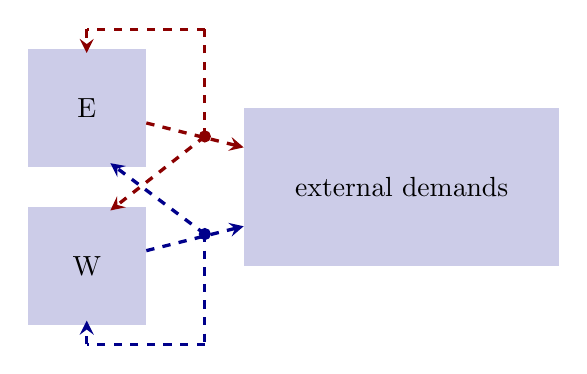
\begin{tikzpicture}[node distance=2cm]
\node (E) [E] {E};
\node (W) [W, below of=E] {W};
\node (ED) [ED, right of=W, xshift=2cm, yshift=1cm] {external demands};
\draw [arrowred] (E) -- (ED);
\draw [arrowblue] (W) -- (ED);
\filldraw[DarkRed] (1.5,-0.36) circle (2pt);
\filldraw[DarkBlue] (1.5,-1.6) circle(2pt);
\draw[DarkRed, very thick, dashed,->, >=stealth] (1.5,-0.36) -- (0.3,-1.3);
\draw[DarkBlue, very thick, dashed,->, >=stealth] (1.5,-1.6) -- (0.3,-0.7);
\draw[DarkRed, very thick, dashed] (1.5,-0.36) -- (1.5,1);
\draw[DarkBlue, very thick, dashed] (1.5,-1.6) -- (1.5,-3);
\draw[DarkRed, very thick, dashed] (1.5,1) -- (0,1);
\draw[DarkBlue, very thick, dashed] (1.5,-3) -- (0,-3);
\draw[DarkRed, very thick, dashed,->, >=stealth] (0,1) -- (0,0.7);
\draw[DarkBlue, very thick, dashed,->, >=stealth] (0,-3) -- (0,-2.7);
\end{tikzpicture}
%\end{column}

%\begin{column}{.45\textwidth}
%%  ENUMERATE
\end{center} 

\begin{itemize}
    \item<1-> this economy contains two sectors: electricity (E), and water (W)
    \item<2-> the \textit{external demands} do not produce E and W
    \item<3-> how might we represent this economy with a set of linear equations?
\end{itemize}

}


\frame{\frametitle{The Leontif Model: Output Vector}
Suppose economy has $N$ sectors, with outputs measured by  $ \vec x \in \mathbb R^N$.  
\begin{align*} 
    \vec x & = \text{output vector} \\
    x_i &= \text{entry } i \text{ of vector } \vec x \\
    &= \text{number of units produced by sector } i
\end{align*}



}


\frame{\frametitle{The Leontif Model: Internal Consumption}

    The \Emph{consumption matrix}, $C$, describes how units are consumed by sectors to produce output. 
    
    \vspace{12pt}
    
    Two equivalent ways of defining entries of $C$.
    \begin{itemize}
        \item<2-> sector $i$ \Emph{sends} a proportion of its units to sector $j$, call it $ c _{i,j}x_i$
        \item<3-> sector $j$ \Emph{requires} a proportion of the units created by sector $i$, call it $ c _{i,j}x_i$
    \end{itemize}
    
    \vspace{12pt}
    
    \onslide<4->{
    Entries of $C$ are $c _{i,j}$, with $c _{i,j} \in[0,1]$, and 
    } 
    \onslide<5->{
    \begin{align*} 
        C\vec x &= \text{units consumed} \\
        \vec x - C\vec x &= \text{units left after internal consumption}
    \end{align*}
    }

}





\frame{\frametitle{Example With Three Sectors}

    An economy contains three sectors, E, W, M. 
    
    \vfill 
    
    For every 100 units of output, 
    \begin{itemize} 
    \item E requires 20 units from E, 10 units from W, and 10 units from M
    \item W requires 0 units from E, 20 units from W, and 10 units from M
    \item M requires 0 units from E, 0 units from W, and 20 units from M
    \end{itemize}
    
    \vfill 
    
    \pause 
    
    If the output vector is $\vec x = \spalignmat{x_E;x_W;x_M}$, construct the consumption matrix for this economy. 

}





\frame{\frametitle{Sketching a Graph for the Economy}
    
    Although not strictly necessary, it can help to sketch the graph for the economy. 
    \begin{center}
    \begin{tikzpicture}
    \begin{scope}[->,>=stealth',shorten >=1pt,auto,node distance=2.2cm,
      thick,main node/.style={circle,fill=DarkBlue!20,draw,font=\sffamily\Large\bfseries}]
        \node[main node] (1) {E};
        \node[main node] (2) [right of=1] {W};
        \node[main node] (3) [below of=2] {M};
        \path[every node/.style={font=\sffamily\small}]
        (1) edge [loop left] node {20\%} (1)
        (2) edge node [above] {10\%} (1)
            edge [loop right] node {20\%} (2)
        (3) edge [bend left] node [above right] {10\%} (1)
            edge node [right] {10\%} (2)
            edge [loop right] node {20\%} (3);
    \end{scope}
    \end{tikzpicture}  
    \end{center}
}
    
  


\frame{\frametitle{Solution: Creating $C$}

    Our consumption matrix is
    $$C = \frac{1}{10} \spalignmat{2 0 0;1 2 0; 1 1 2} $$
    Note: 
    \begin{itemize}
        \item total output for each sector is the sum along the outgoing edges for each sector, which generates rows of $C$
        \item elements of $C$ represent percentages with no units, they have values between 0 and 1
        \item our output vector has units
    \end{itemize}

}

\frame{\frametitle{The Leontif Model: Demand}

\vspace{6pt}

There is also an external demand given by $ \vec d \in \mathbb R^N$. We ask if there is an $\vec x$ such that
$$\vec x -  C \vec x = \vec d$$
We can re-write this as 
$$ (I - C)\vec x = \vec d$$
This matrix equation is the \Emph{Leontief Input-Output Model}. Solving for $\vec x$ gives the output that meets external demand exactly.


}  

\frame{\frametitle{Example Revisited}

    Now suppose there is an external demand: what production level is required to satisfy a final demand of 80 units of E, 70 units of W, and 160 units of M?
    
    \vspace{4pt}
    \begin{center}
\begin{tikzpicture}
\begin{scope}[->,>=stealth',shorten >=1pt,auto,node distance=3.4cm,
  thick,main node/.style={circle,fill=DarkBlue!20,draw,font=\sffamily\Large\bfseries}]
  \node[main node] (1) {E};
  \node[main node] (2) [right of=1] {W};
    \node[main node] (3) [below of=2] {M};
    \node[main node] (4) [below of=1] {D};
  \path[every node/.style={font=\sffamily\small}]
    (1) edge [loop left] node {20\%} (1)
        edge [DarkRed] node[left] {80 units} (4)
    (2) edge node [above] {10\%} (1)
        edge [loop right] node {20\%} (2)
        edge [bend right, DarkRed] node[above left] {} (4)
    (3) edge [bend left] node [above right] {10\%} (1)
        edge node [right] {10\%} (2)
        edge [loop right] node {20\%} (3)
        edge [DarkRed] node[below] {160 units}  (4);
\end{scope}
        \draw (2,-1.2) node [DarkRed] {70 units};
        \end{tikzpicture}  
            \end{center}
}
    

\frame{\frametitle{Solution}
The production level would be found by solving:
    \begin{align*}
    (I - C)\vec x &= \vec d \\
        \frac{1}{10} \spalignmat{8 0 0;-1 8 0; -1 -1 8} \vec x &= \spalignmat{80;70;160} \\
        8x_1 &= 800 \quad \Rightarrow \quad x_1 = 100\\
        -x_1 + 8x_2 &= 700 \quad \Rightarrow \quad x_2 = 100 \\
        -x_1 - x_2 + 8x_3 &= 1600 \quad
        \Rightarrow \quad x_3 = 1800/8 = 225
    \end{align*}
    \pause
    The output that balances demand with internal consumption is $\vec x = \spalignmat{100;100;225 }.$
}



% \frame{\frametitle{The Importance of $(I-C)^{-1}$}

% For the example above
% \begin{equation*}
% (I-C) ^{-1} \approx \spalignmat{1.25,0,0;0.15,1.25,0;0.18,0.17,1.25}
% \end{equation*}


% The entries of $ (I - C) ^{-1} = B$ have this meaning:  if the final demand vector $ \vec d$ increases by one unit in the $ j^{th}$ place, the column vector $ b_j$ is the additional output required from other sectors.  


% \bigskip 
% So to meet an increase in demand for M by one unit, requires 1.25 of one additional units from M to meet internal consumption.  

% }







\frame{\frametitle{Summary}

    \SummaryLine \vspace{4pt}
    \begin{itemize}\setlength{\itemsep}{8pt}
        \item setting up and solving Leontif input-output models
    \end{itemize}
    
    \vspace{4pt}
    
    This video explored an application of systems of equations.
    



}



\frame{
}
